\documentclass[hidelinks,12pt]{article}
\usepackage[left=0.25cm,top=1cm,right=0.25cm,bottom=1cm]{geometry}
%\usepackage[landscape]{geometry}
\textwidth = 20cm
\hoffset = -1cm
\usepackage[utf8]{inputenc}
\usepackage[spanish,es-tabla]{babel}
\usepackage[autostyle,spanish=mexican]{csquotes}
\usepackage[tbtags]{amsmath}
\usepackage{nccmath}
\usepackage{amsthm}
\usepackage{amssymb}
\usepackage{mathrsfs}
\usepackage{graphicx}
\usepackage{subfig}
\usepackage{standalone}
\usepackage[outdir=./Imagenes/]{epstopdf}
\usepackage{siunitx}
\usepackage{physics}
\usepackage{color}
\usepackage{float}
\usepackage{hyperref}
\usepackage{multicol}
%\usepackage{milista}
\usepackage{anyfontsize}
\usepackage{anysize}
%\usepackage{enumerate}
\usepackage[shortlabels]{enumitem}
\usepackage{capt-of}
\usepackage{bm}
\usepackage{relsize}
\usepackage{placeins}
\usepackage{empheq}
\usepackage{cancel}
\usepackage{wrapfig}
\usepackage[flushleft]{threeparttable}
\usepackage{makecell}
\usepackage{fancyhdr}
\usepackage{tikz}
\usepackage{bigints}
\usepackage{scalerel}
\usepackage{pgfplots}
\usepackage{pdflscape}
\pgfplotsset{compat=1.16}
\spanishdecimal{.}
\renewcommand{\baselinestretch}{1.5} 
\renewcommand\labelenumii{\theenumi.{\arabic{enumii}})}
\newcommand{\ptilde}[1]{\ensuremath{{#1}^{\prime}}}
\newcommand{\stilde}[1]{\ensuremath{{#1}^{\prime \prime}}}
\newcommand{\ttilde}[1]{\ensuremath{{#1}^{\prime \prime \prime}}}
\newcommand{\ntilde}[2]{\ensuremath{{#1}^{(#2)}}}

\newtheorem{defi}{{\it Definición}}[section]
\newtheorem{teo}{{\it Teorema}}[section]
\newtheorem{ejemplo}{{\it Ejemplo}}[section]
\newtheorem{propiedad}{{\it Propiedad}}[section]
\newtheorem{lema}{{\it Lema}}[section]
\newtheorem{cor}{Corolario}
\newtheorem{ejer}{Ejercicio}[section]

\newlist{milista}{enumerate}{2}
\setlist[milista,1]{label=\arabic*)}
\setlist[milista,2]{label=\arabic{milistai}.\arabic*)}
\newlength{\depthofsumsign}
\setlength{\depthofsumsign}{\depthof{$\sum$}}
\newcommand{\nsum}[1][1.4]{% only for \displaystyle
    \mathop{%
        \raisebox
            {-#1\depthofsumsign+1\depthofsumsign}
            {\scalebox
                {#1}
                {$\displaystyle\sum$}%
            }
    }
}
\def\scaleint#1{\vcenter{\hbox{\scaleto[3ex]{\displaystyle\int}{#1}}}}
\def\bs{\mkern-12mu}


\title{Transformada de Fourier} \vspace{-3ex}
\author{M. en C. Gustavo Contreras Mayén}
\date{ }
\newcommand{\Cancel}[2][black]{{\color{#1}\cancel{\color{black}#2}}}
\begin{document}
\vspace{-4cm}
\maketitle
\fontsize{14}{14}\selectfont
\tableofcontents
\newpage

%Referencia. Patra - Integral transforms and their applications. Sec. 1.4
\section{Las transformadas de Fourier.}

Una vez revisado el material introductorio, podemos definir la \emph{transformada de Fourier} (TF) de una función continua por partes $f(x) \in P^{1} (R)$ y tal que $f(x) \in A_{1} (R)$. La transformada se define por:
\begin{align}
\begin{aligned}[b]
F \big[ f(x); x \to \xi \big] &= F \big[f(x) \big] \\[0.5em]
&= F(\xi) = \overline{f} (\xi) = \\[0.5em] 
&= \dfrac{1}{\sqrt{2 \, \pi}} \int_{-\infty}^{+\infty} f(x) \, \exp(i \, \xi \, x) \dd{x}
\end{aligned}
\label{eq:ecuacion_01_12}
\end{align}
y también:
\begin{align}
f(x) = F^{-1} \big[ F(\xi) \big] = \dfrac{1}{\sqrt{2 \, \pi}} \int_{-\infty}^{+\infty} F(\xi) \, \exp(-i \, \xi \, x) \dd{\xi}
\label{eq:ecuacion_01_13}
\end{align}
en un punto continuo de $f(x)$.
\par
La función $F(\xi)$ en la ec. (\ref{eq:ecuacion_01_12}) es la \emph{transformada de Fourier} de $f(x)$, mientras que $f(x)$ en la ec. (\ref{eq:ecuacion_01_13}) es la llamada \emph{transformada inversa de Fourier} de $F(\xi)$.
\par
Algunos autores definen la transformada de Fourier  (ec. \ref{eq:ecuacion_01_12}) y la transformada inversa (ec. \ref{eq:ecuacion_01_13}) respectivamente como:
\begin{align}
F \big[ f(x); x \to \xi \big] = F(\xi) = \int_{-\infty}^{+\infty} f(x) \, \exp(i \, \xi \, x) \dd{x} \label{eq:ecuacion_01_14} \\[0.5em]
f(x) = \dfrac{1}{2 \, \pi} \int_{-\infty}^{+\infty} F(\xi) \, \exp(-i \, \xi \, x) \dd{\xi}
\label{eq:ecuacion_01_15}
\end{align}

En un punto de discontinuidad de $x \in R$, el lado izquierdo de las ecs. (\ref{eq:ecuacion_01_13}) y (\ref{eq:ecuacion_01_15}), toman la forma:
\begin{align*}
\dfrac{1}{2} \big[ f(x + 0) + f(x - 0) \big]
\end{align*}
en lugar de $f(x)$.
\par
De las definiciones de las transformadas de Fourier y de la transformada inversa de Fourier, es posible escribir de la ec. (\ref{eq:ecuacion_01_12})
\begin{align*}
F(\xi) = F \big[f(x) \big] = F \big[ F^{1} (F(\xi))\big] \hspace{0.2cm} &\Rightarrow \hspace{0.2cm} F \, F^{-1} \big[ F(\xi)\big] \equiv I \big[ F(\xi)\big] \\[0.5em]
&\Rightarrow \hspace{0.2cm} F \, F^{-1} = I
\end{align*}
que es un operador de identidad, entonces $F$ y $F^{-1}$ son los operadores de Fourier y
su operador inverso respectivamente, y de la ec. (\ref{eq:ecuacion_01_13}):
\begin{align}
\begin{aligned}[b]
f(x) = F^{-1} \big[F(\xi)\big] = F^{-1} \big[F(f(x))\big] &= F^{-1} \, F \big[f(x)\big] = I \big[f(x)\big] \\[0.5em]
&\Rightarrow \hspace{0.2cm} F^{-1} \, F = I
\end{aligned}
\label{eq:ecuacion_01_16}
\end{align}
Por lo que en una notación de operador:
\begin{align*}
F \, F^{-1} = F^{-1} \, F = I
\end{align*}
Esto demuestra que los operadores $F$ y $F^{-1}$ son conmutativos.

\subsection{Transformadas seno y coseno de Fourier.}

Consideremos que la función\footnote{Para las definiciones de este tipo de funciones, revisa las notas de Introducción a las Transformadas Integrales.} $f(x)$ sea una función \emph{impar} de $x \in R$, perteneciente además a las clases $P^{1} (R)$ y $A_{1} (R)$. Tenemos claramente que $f(-x) = - f(x)$. 
\par
De la ec. (\ref{eq:ecuacion_01_12}):
\begin{align}
\begin{aligned}[b]
F \big[ f(x); x \to \xi \big] = F(\xi) &= \dfrac{1}{\sqrt{2 \, \pi}} \int_{0}^{\infty} f(x) \big[\exp(i \xi x) {-} \exp(-i \xi x) \big] \dd{x} = \\[0.5em]
&= i \, \sqrt{\dfrac{2}{\pi}} f(x) \, \sin \xi \, x \dd{x} = \\[0.5em]
&\equiv i \, F_{s} (\xi)
\end{aligned}
\label{eq:ecuacion_01_17}
\end{align}
donde:
\begin{align}
F_{s} (\xi) = \sqrt{\dfrac{2}{\pi}} f(x) \, \sin \xi \, x \dd{x}
\label{eq:ecuacion_01_18}
\end{align}
La ec. (\ref{eq:ecuacion_01_18}) define la \emph{transformada seno de Fourier} de la función $f(x)$.
\par
Su conexión con la transformada de Fourier, está dada por la ec. (\ref{eq:ecuacion_01_17}) donde $f (x)$ es una función impar de $x \in R$. La expresión para la transformada inversa de (\ref{eq:ecuacion_01_18}) se define por:
\begin{align}
f(x) = \sqrt{\dfrac{2}{\pi}} \int_{0}^{\infty} F_{s}(\xi) \, \sin \xi \, x \dd{\xi}
\label{eq:ecuacion_01_19}
\end{align}
Sea ahora una función par $f(x)$ de $x \in R$, además de que pertenece a la clases $P^{1}(R)$ y $A_{1}(R)$. Entonces: $f(-x) = f(x)$, por lo tanto, por la ec. (\ref{eq:ecuacion_01_12}):
\begin{align}
\begin{aligned}[b]
F \big[ f(x); x \to \xi \big] = F(\xi) &= \dfrac{1}{\sqrt{2 \, \pi}} \int_{0}^{\infty} f(x) \big[\exp(i \xi x) {+} \exp(-i \xi x) \big] \dd{x} = \\[0.5em]
&= i \, \sqrt{\dfrac{2}{\pi}} f(x) \, \cos \xi \, x \dd{x} = \\[0.5em]
&\equiv i \, F_{c} (\xi)    
\end{aligned}
\label{eq:ecuacion_01_20}
\end{align}
donde:
\begin{align}
F_{c} (\xi) = \sqrt{\dfrac{2}{\pi}} f(x) \, \cos \xi \, x \dd{x}
\label{eq:ecuacion_01_21}
\end{align}
La ec. (\ref{eq:ecuacion_01_21}) define la \emph{transformada coseno de Fourier} de la función $f(x)$.
\par
Su conexión con la transformada de Fourier, está dada por la ec. (\ref{eq:ecuacion_01_20}) donde $f (x)$ es una función par de $x \in R$. La expresión para la transformada inversa de (\ref{eq:ecuacion_01_21}) se define por:
\begin{align}
f(x) = \sqrt{\dfrac{2}{\pi}} \int_{0}^{\infty} F_{c}(\xi) \, \cos \xi \, x \dd{\xi}
\label{eq:ecuacion_01_22}
\end{align}

\subsection{Propiedad de linealidad.}

Si $c_{1}$ y $c_{2}$ son constantes, se tiene entonces que:
\begin{enumerate}[\thesubsection .1)]
\item \label{inciso_01} $F \big[c_{1} \, f_{1} (x) + c_{2} \, f_{2} (x)\big] = c_{1} \, F \big[ f_{1} (x)\big] + c_{2} \, F \big[ f_{2} (x)\big]$
\item $F_{s} \big[c_{1} \, f_{1} (x) + c_{2} \, f_{2} (x)\big] = c_{1} \, F_{s} \big[ f_{1} (x)\big] + c_{2} \, F_{s} \big[ f_{2} (x)\big]$
\item $F_{c} \big[c_{1} \, f_{1} (x) + c_{2} \, f_{2} (x)\big] = c_{1} \, F_{c} \big[ f_{1} (x)\big] + c_{2} \, F_{c} \big[ f_{2} (x)\big]$
\end{enumerate}
La demostración se sigue de la definición de la transformada de Fourier de la ec. (\ref{eq:ecuacion_01_12}), en el caso del inciso (\ref{inciso_01}, se tiene que: 
\begin{align*}
&F \big[ c_{1} \, f_{1} (x) + c_{2} \, f_{2} (x) ; x \to \xi \big] = \\[0.5em]
&= \dfrac{1}{\sqrt{2 \, \pi}} \int_{-\infty}^{\infty} \big[ c_{1} \, f_{1} (x) + c_{2} \, f_{2} (x) \big] \, \exp(i \xi x) \dd{x} = \\[0.5em]
&= c_{1} \, \dfrac{1}{\sqrt{2 \, \pi}} \int_{-\infty}^{\infty} f_{1}(x) \, \exp(i \xi x) \dd{x} + c_{2} \, \dfrac{1}{\sqrt{2 \, \pi}} \int_{-\infty}^{\infty} f_{2}(x) \, \exp(i \xi x) \dd{x} = \\[0.5em]
&= c_{1} \, F \big[ f_{1} (x) ; x \to \xi \big] + c_{2} \, F \big[ f_{2} (x) ; x \to \xi \big]
\end{align*}
La demostración de los otros dos incisos es análoga.

\subsection{Propiedad de cambio de escala.}

\begin{enumerate}[\thesubsection .1)]
\item Si $F \big[ f(x); x \to \xi \big] = F(\xi)$, entonces:
\begin{align*}
F \big[ f(a \, x); x \to \xi \big] = \dfrac{1}{a} \, F \left( \dfrac{\xi}{a} \right)
\end{align*}
\item \label{inciso_01_06_01} Si $F_{s} \big[f(x)\big] = F_{s}(\xi)$, entonces:
\begin{align*}
F_{s} \big[f(a \, x)\big] = \dfrac{1}{a} \, F_{s} \left( \dfrac{\xi}{a} \right)
\end{align*}
\item Si $F_{c} \big[f(x); x \to \xi\big] = F_{c}(\xi)$, entonces:
\begin{align*}
F_{c} \big[f(a \, x); x \to \xi \big] = \dfrac{1}{a} \, F_{c} \left( \dfrac{\xi}{a} \right)
\end{align*}
\end{enumerate}

La demostración del inciso (\ref{inciso_01_06_01} se sigue de la definición:
\begin{align*}
F_{s} \big[f(x); x \to \xi \big] = \sqrt{\dfrac{2}{\pi}} \int_{0}^{\infty} f(x) \, \sin \xi \, x \dd{\xi} = F_{s} (\xi)
\end{align*}
por lo que:
\begin{align*}
&F_{s} \big[f(a \, x); x \to \xi \big] = \sqrt{\dfrac{2}{\pi}} \int_{0}^{\infty} f(a \, x) \, \sin \xi \, x \dd{\xi} = \\[0.5em]
&= \dfrac{1}{a} \, \sqrt{\dfrac{2}{\pi}} \int_{0}^{\infty} f(t) \sin \left( \dfrac{\xi}{a} \, t \right) \dd{t} = \\[0.5em]
&= \dfrac{1}{a} \, F_{s} \left( \dfrac{\xi}{a} \right)
\end{align*}
La demostración de los otros dos incisos, se sigue de la misma manera, ocupando la definición de la transformada de Fourier y la transformada coseno de Fourier.

\subsection{Propiedad de desplazamiento.}

Si $F(\xi)$ es la transformada de Fourier de $f(x)$ en $R$, entonces la transformada de Fourier de $f(x - a)$ es:
\begin{align*}
f(x - a) = \exp(i \, \xi \, a) \, F(\xi)
\end{align*}

Comenzamos la demostración de la propiedad de desplazamiento a partir de la definición:
\begin{align*}
F(\xi) = \dfrac{1}{\sqrt{2 \, \pi}} \int_{-\infty}^{+\infty} f(x) \, \exp(i \, \xi \, x) \dd{x} = F \big[f(x); x \to \xi \big]
\end{align*}
Por lo tanto:
\begin{align*}
F \big[f(x - a); x \to \xi \big] &= \dfrac{1}{\sqrt{2 \, \pi}} \int_{-\infty}^{+\infty} f(x - a) \, \exp(i \, \xi \, x) \dd{x} \\[0.5em]
&= \dfrac{1}{\sqrt{2 \, \pi}} \int_{-\infty}^{+\infty} f(t) \, \exp(i \, \xi (t + a)) \dd{t} \\[0.5em]
&= \exp(i \, \xi \, a) \, \dfrac{1}{\sqrt{2 \, \pi}} \int_{-\infty}^{+\infty} f(t) \, \exp(i \, \xi \, t) \dd{t} \\[0.5em]
&= \exp(i \, \xi \, a) \, F (\xi) 
\end{align*}

\subsection{El teorema de modulación.}

\textbf{Teorema:} Si $F \big[f(x); x \to \xi \big] = F(\xi)$, entonces:
\begin{align*}
F \big[f(x) \, \cos a \, x; x \to \xi \big] = \dfrac{1}{2} \big[F(\xi + a) + F(\xi - a) \big]
\end{align*}

\textbf{Demostración:}
\\
Ya que se tiene:
\begin{align*}
F \big[f(x); x \to \xi \big] = F(\xi) = \dfrac{1}{\sqrt{2 \, \pi}} \int_{-\infty}^{+\infty} f(x) \, \exp(i \, \xi \, x) \dd{x}
\end{align*}
entonces:
\begin{align*}
F \big[f(x); x \to \xi \big] &= \dfrac{1}{\sqrt{2 \, \pi}} \int_{-\infty}^{+\infty} f(x) \, \dfrac{\exp(i \, a \, x) + \exp(-i \, a \, x)}{2} \, \exp(i \, \xi \, x) \dd{x} = \\[0.5em]
&= \dfrac{1}{2} \left[ \dfrac{1}{\sqrt{2 \, \pi}} \int_{-\infty}^{+\infty} f(x) \, \exp(i \, (\xi + a) \, x)  \dd{x} + \right. \\[0.5em]
&+ \left. \dfrac{1}{\sqrt{2 \, \pi}} \int_{-\infty}^{+\infty} f(x) \, \exp(i \, (\xi - a) \, x)  \dd{x} \right] = \\[0.5em]
&= \big[ F(\xi + a) + F (\xi - a \big]
\end{align*}

Otras tres partes del teorema son:
\begin{enumerate}[label=\alph*)]
\item Si $F_{s} \big[f(x); x \to \xi \big] = F_{s} (\xi)$, entonces:
\begin{align*}
F_{s} \big[f(x) \, \cos a \, x; x \to \xi \big] = \dfrac{1}{2} \big[F_{s} (\xi +  a) + F_{s} (\xi - a) \big]
\end{align*}
\item Si $F_{s} \big[f(x); x \to \xi \big] = F_{s} (\xi)$, entonces:
\begin{align*}
F_{c} \big[f(x) \, \sin a \, x; x \to \xi \big] = \dfrac{1}{2} \big[F_{s} (\xi +  a) - F_{s} (\xi - a) \big]
\end{align*}
\item Si $F_{c} \big[f(x); x \to \xi \big] = F_{c} (\xi)$, entonces:
\begin{align*}
F_{s} \big[f(x) \, \sin a \, x; x \to \xi \big] = \dfrac{1}{2} \big[F_{c} (\xi -  a) - F_{c} (\xi + a) \big]
\end{align*}
\end{enumerate}

Estos resultados pueden demostrarse de manera similar como se hizo en el primer caso al reemplazar $\cos a \, x$ y $\sin a \, x$ por sus formas exponenciales en las definiciones de las transformadas correspondientes del lado izquierdo.

\subsection{Evaluación de integrales mediante transformadas inversas.}

Por definiciones de la transformada de Fourier y su transformada inversa en las ecs. (\ref{eq:ecuacion_01_12}), (\ref{eq:ecuacion_01_13}), (\ref{eq:ecuacion_01_17}), (\ref{eq:ecuacion_01_19}), (\ref{eq:ecuacion_01_21}) y (\ref{eq:ecuacion_01_22}), podemos emplear esos resultados para evaluar ciertas integrales que involucran funciones trigonométricas. 
\bigskip

\noindent
\textbf{Ejemplo 1.}
\\
En primer lugar consideramos:
\begin{align*}
I_{1} = \int_{0}^{\infty} \exp (-b \, x) \, \cos a \, x \dd{x}, \hspace{1cm} I_{2} = \int_{0}^{\infty} \exp (-b \, x) \, \sin a \, x \dd{x}
\end{align*}
Integrando por partes podemos evaluar $I_{1}$ e $I_{2}$ como:
\begin{align*}
I_{1} = \dfrac{b}{a^{2} + b^{2}},  \hspace{1.5cm} I_{2} = \dfrac{a}{a^{2} + b^{2}}
\end{align*}
Estos resultados implican que si hacemos $f(x) = \exp(-b \, x)$, entonces las transformadas seno y coseno están dadas por:
\begin{align*}
F_{c} \big[\exp(-b \, x); x \to \xi \big] &= \sqrt{\dfrac{2}{\pi}} \, \dfrac{b}{\xi^{2} + b^{2}} \\[0.5em]
F_{s} \big[\exp(-b \, x); x \to \xi \big] &= \sqrt{\dfrac{2}{\pi}} \, \dfrac{\xi}{\xi^{2} + b^{2}}
\end{align*}
Al sustituir éstas expresiones en las ecs. (\ref{eq:ecuacion_01_19}) y (\ref{eq:ecuacion_01_22}), tenemos que:
\begin{align*}
\int_{0}^{\infty} \dfrac{\cos \xi \, x}{\xi^{2} + b^{2}} \dd{\xi} &= \dfrac{\pi}{2 \, b} \, \exp(-b \, x) \\[1em]
\int_{0}^{\infty} \dfrac{\xi \, \sin \xi \, x}{\xi^{2} + b^{2}} \dd{\xi} &= \dfrac{\pi}{2} \, \exp(-b \, x)
\end{align*}
\bigskip

\noindent
\textbf{Ejemplo 2.}
\\
Si hacemos que la función $f(x)$ sea tal que:
\begin{align*}
f(x) = \begin{cases}
1, & 0 < x < a \\[0.5em]
0, & x > a
\end{cases}
\end{align*}
entonces:
\begin{align*}
F_{c}(\xi) = \dfrac{2}{\pi} \int_{0}^{a} 1 \, \cos \xi \, x \dd{x} = \sqrt{\dfrac{2}{\pi}} \, \dfrac{\sin \xi \, a}{\xi}
\end{align*}
para así obtener:
\begin{align*}
\dfrac{2}{\pi} \int_{0}^{a} \, \dfrac{\sin \xi \, a}{\xi} \, \cos \xi \, x \dd{x} = \begin{cases}
1, & \mbox{si } 0 < x < a \\[0.5em]
0, & \mbox{si } x \geq a
\end{cases}
\end{align*}

\subsection{Transformada de Fourier de algunas funciones particulares.}

Consideremos la siguiente función \enquote{escalón} $f(x)$, definida por:
\begin{align*}
f(x) = \begin{cases}
0, & x < 0 \\[0.5em]
1, & x > 0
\end{cases}
\end{align*}

Esta función se conoce como la \emph{función de paso unitario de \textbf{Heaviside}}, que se representa como $H(x)$. Entonces se tiene que:
\begin{align*}
H(x) = \begin{cases}
0, & x < 0 \hspace{0.3cm} (\mbox{o también para } x \leq 0 ) \\[0.5em]
1, & x > 0
\end{cases}
\end{align*}

Casi todas las funciones escalonadas se pueden expresar como una combinación de funciones escalonadas unitarias de Heaviside. Por ejemplo:
\begin{align*}
f(x) = \begin{cases}
1, & \abs{x} < a \\[0.5em]
0, & \mbox{de otra manera}
\end{cases}
\end{align*}
es equivalente a:
\begin{align*}
f(x) = H(x + a) - H(x- a) \equiv H(a - \abs{x})
\end{align*}

La función escalón:
\begin{align*}
f(x) = \begin{cases}
k, & x > a \\[0.5em]
0, & \mbox{de otra manera}
\end{cases}
\end{align*}
es equivalente a:
\begin{align*}
f(x) = k \, H(x - a) \hspace{0.3cm} \forall \, x
\end{align*}
\bigskip

\noindent
\textbf{Ejemplo 1.}
\\
Evaluar la transformada de Fourier de:
\begin{align*}
H(x + a) - H(x - a)
\end{align*}
Por definición:
\begin{align*}
&F \big[H(x + a) - H(x - a); x \to \xi\big] = \\[0.5em]
&= \dfrac{1}{\sqrt{2\, \pi}} \int_{0}^{\infty} \exp(i \, \xi \, x) \big[H(x + a) - H(x - a)\big] \dd{x} = \\[0.5em]
&= \dfrac{1}{\sqrt{2\, \pi}} \int_{-a}^{a} \exp(i \, \xi \, x) \dd{x} = \\[0.5em]
&= \dfrac{1}{\sqrt{2\, \pi}} \, \left[ \dfrac{\exp(i \, \xi \, x)}{i \, \xi} \right] \eval_{-a}^{a} = \\[0.5em]
&= \dfrac{1}{\sqrt{2\, \pi} \, i \, \xi} \, \big[\exp(i \, \xi \, a) - \exp(-i \, \xi \, ) \big] = \\[0.5em]
&= \sqrt{\dfrac{2}{\pi}} \dfrac{\sin a \, \xi}{\xi}
\end{align*}

Por lo que, usando la transformada de Fourier inversa, se obtiene:
\begin{align*}
\dfrac{1}{\sqrt{2 \, \pi}} \, \int_{-\infty}^{+\infty} \sqrt{\dfrac{2}{\pi}} \, \dfrac{\sin a \, \xi}{\xi} \,  \exp(- i \, \xi \, x) \dd{\xi}  = H(x + a) - H(x- a)
\end{align*}
Este resultado implica que:
\begin{align*}
\dfrac{1}{\pi} \int_{-\infty}^{+\infty} \dfrac{\sin a \, \xi}{\xi} \, \big[\cos \xi \, x - i \, \sin \xi \, x \big] \dd{x} = H(x + a) - H(x - a)
\end{align*}
es decir:
\begin{align*}
\int_{-\infty}^{+\infty} \dfrac{\sin a \, \xi}{\xi} \, \cos \xi \, x \dd{x} &= \pi \, \big[H(x + a) - H(x - a)\big]  = \\[0.5em]
&= \begin{cases}
\pi, & \mbox{para  } \abs{x} < a \\[0.5em]
0, & \mbox{para  } \abs{x} > a
\end{cases}
\end{align*}
Haciendo que $x = 0$ y $a = 1$, en la expresión anterior tenemos que:
\begin{align*}
\int_{-\infty}^{+\infty} \dfrac{\sin a \, \xi}{\xi} = \pi
\end{align*}
lo que implica que:
\begin{align*}
\int_{0}^{\infty} \dfrac{\sin a \, \xi}{\xi} = \dfrac{\pi}{2}
\end{align*}
y además:
\begin{align*}
\int_{-\infty}^{+\infty} \dfrac{\sin a \, \xi \, \sin \xi \, x}{\xi} = 0
\end{align*}

\subsection{Convolución de dos funciones integrables.}

La convolución\footnote{El término convolución no aparece en el diccionario de la Real Academia Española; su empleo matemático es una castellanización del término inglés \enquote{Convolution} (twist together) cuyo significado más idóneo es: \enquote{retorcido conjunto}. En alemán es\enquote{faltung} (doblar), y en francés, \enquote{composition}.} de dos funciones integrables $f(x)$ y $g(x)$, donde \hfill \break
$-\infty < x < \infty$ se escribe y se define como:
\begin{align}
f * g = \dfrac{1}{\sqrt{2 \, \pi}} \int_{-\infty}^{+\infty} f(x - u) \, g(u) \dd{u}
\label{eq:ecuacion_01_23}
\end{align}

La convolución tiene varias propiedades como:
\begin{align*}
f * (\lambda \, g) &= (\lambda \, f) * g = \lambda (f * g), \hspace{1cm} \lambda = \mbox{constante} \\[0.5em]
f * g &= g * f \hspace{1.5cm} \mbox{propiedad conmutativa} \\[0.5em]
f * (g + h) &= f * g + f * h
\end{align*}
que se pueden verificar fácilmente directamente desde la definición (\ref{eq:ecuacion_01_23}). \hfill \break 
Además, si tanto $f (x)$ como $g (x)$ pertenecen a las clases $C^{1} (R)$ y $A_{1} (R)$, entonces también lo hace su convolución $h (x) = f * g$, ya que:
\begin{align*}
\sqrt{2 \, \pi} \, \int_{-\infty}^{+\infty} \abs{h(x)} \dd{x} &= \int_{-\infty}^{+\infty} \dd{x} \, \abs{\int_{-\infty}^{+\infty} f(u) g(x - u) \dd{u}} < \\[0.5em]
&< \int_{-\infty}^{+\infty} \dd{x} \, \int_{-\infty}^{+\infty} \abs{f(u) g(x - u)} \dd{u} = \\[0.5em]
&= \int_{-\infty}^{+\infty} \abs{f(u)} \dd{u} \, \int_{-\infty}^{+\infty} \abs{g(x - u)} \dd{u} \\[0.5em]
\Rightarrow \int_{-\infty}^{+\infty} \abs{h(x)} \dd{x} &< \dfrac{1}{\sqrt{2 \, \pi}} \int_{-\infty}^{+\infty} \abs{f(u)} \dd{u} \, \int_{-\infty}^{+\infty} \abs{g(\nu)} \dd{\nu}
\end{align*}
y el resultado se sigue del hecho que tanto $f(x)$ y $g(x)$ pertenecen a la clase $A_{1}(R)$.
\par
Nuevamente $(f * g) * h = f * (g * h)$ es cierto haciendo una revisión directa. Por lo tanto la propiedad de convolución es también asociativa.
\par
Ahora discutiremos la transformada de Fourier de la convolución de un par de funciones, con el nombre de convolución o teorema de Faltung o Faltung para la Transformada de Fourier.

\subsection{Teorema de convolución para la Transformada de Fourier.}

\textbf{Teorema.}

La transformada de Fourier de $f(x)$ y $g(x)$, ambas funciones pertenecen a las clases $C^{1}(R)$ y $A_{1}(R)$, es el producto de las transformadas de Fourier de $f(x)$ y $g(x)$. Es decir:
\begin{align*}
F \big[f * g; x \to \xi \big] &= F(\xi) \, G(\xi) \\[0.5em]
\mbox{donde } \hspace{0.4cm} F(\xi) &= \dfrac{1}{\sqrt{2 \, \pi}} \int_{-\infty}^{\infty} f(x) \, \exp(i \, \xi, x) \dd{x} \hspace{0.3cm} \mbox{y} \\[0.5em]
G(\xi) &= \dfrac{1}{\sqrt{2 \, \pi}} \int_{-\infty}^{\infty} g(x) \, \exp(i \, \xi, x) \dd{x}
\end{align*}

\textbf{Demostración: }

Ya que tanto $f(x)$ como $g(x)$ pertenecen ambas a las clases $C^{1}(R)$ y $A_{1}(R)$, se tiene que $f * g$ también pertenece a las clases $C^{1}(R)$ y $A_{1}(R)$, por lo que la transformada de Fourier de $f * g$ también existe. Por lo que:
\begin{align}
\hspace*{-0.5cm}
\begin{aligned}[b]
F \big[f * g; x {\to} \xi \big] &= \dfrac{1}{\sqrt{2 \pi}} \int_{-\infty}^{\infty} \! e^{i  \xi x} \dfrac{\dd{x}}{\sqrt{2 \pi}} \int_{-\infty}^{\infty} \! f(x {-} u) g(u) \dd{u} \\[0.5em]
&= \dfrac{1}{2 \pi} \int_{-\infty}^{\infty} \int_{-\infty}^{\infty} \! f(x {-} u) g(u) \exp(i \xi x) \dd{x} \dd{u} = \\[0.5em]
&= \dfrac{1}{2 \pi} \int_{-\infty}^{\infty} g(u) \left[ \int_{-\infty}^{\infty} \! \exp(i \xi x) f(x {-} u) \dd{x} \right] \dd{u} = \\[0.5em]
&= \dfrac{1}{\sqrt{2  \pi}} \int_{-\infty}^{\infty} \! g(u) \exp(i \xi u) \left[ \int_{-\infty}^{\infty} \! \exp(i \xi \nu) f(\nu) \dd{\nu} \right] \dd{u} = \\[0.5em]
&= \dfrac{1}{\sqrt{2 \pi}} \int_{-\infty}^{\infty} \! g(u) \exp(i  \xi u) \cdot F(\xi) \dd{u} \\[1em]
F \big[f * g; x \to \xi \big] &= F(\xi) \, G(\xi)
\end{aligned}
\label{eq:ecuacion_01_24}
\end{align}

Lo que demuestra el teorema.
\\
\bigskip

\textbf{Corolario 1.}

Otra interpretación del teorema de convolución de la ec. (\ref{eq:ecuacion_01_24}) es tal que:
\begin{align}
\begin{aligned}[b]
F^{-1} \, \big[F(\xi) \, G(\xi); \xi \to x\big] &= \dfrac{1}{\sqrt{2 \, \pi}} \int_{-\infty}^{+\infty} f(x - u) \, g(u) \dd{u} \\[0.5em]
\mbox{O}, \hspace{0.4cm} \dfrac{1}{\sqrt{2 \, \pi}} \int_{-\infty}^{+\infty} F(\xi) \, G(\xi) \, \exp(- i \xi x) \dd{\xi} &= \dfrac{1}{\sqrt{2 \pi}} \int_{-\infty}^{+\infty} f(\nu) g(x - \nu) \dd{\nu} \\[0.5em]
&= f * g
\end{aligned}
\label{eq:ecuacion_01_25}
\end{align}

\newpage

\textbf{Corolario 2.}

Del resultado anterior (\ref{eq:ecuacion_01_25}), se tiene que:
\begin{align*}
\dfrac{1}{\sqrt{2 \, \pi}} \int_{-\infty}^{+\infty} F(\xi) \, G(\xi) \, \exp(- i \xi x) \dd{\xi} &= f * g =\\[0.5em]
&= \dfrac{1}{\sqrt{2 \, \pi}} \int_{-\infty}^{+\infty} f(\nu) g(x - \nu) \dd{\nu}
\end{align*}
Haciendo que $x = 0$ en la ecuación anterior, vemos que:
\begin{align}
\int_{-\infty}^{+\infty} F(\xi) \, G(\xi) \dd{\xi} = \int_{-\infty}^{+\infty} f(\nu) g(-\nu) \dd{\nu}
\label{eq:ecuacion_01_26}
\end{align}
\\
\bigskip

\textbf{Corolario 3.}

Sea $f(x) \in R$. Entonces $F(\xi) = F \big[f(x); x \to \xi\big]$ es una función compleja y su conjugado, escrito como $\overline{F}(\xi)$ está dado por:
\begin{align}
\begin{aligned}[b]
\overline{F}(\xi) = \dfrac{1}{\sqrt{2 \, \pi}} \int_{-\infty}^{\infty} f(x) \, \exp(-i \, \xi \, x) \dd{x} &= F^{-1} \, \big[f(x); x \to \xi\big] \\[0.5em]
\mbox{es decir} \hspace{0.5cm} \overline{F} \left\{f(x); x \to \xi \right\} &= F^{-1} F^{-1} \, \big[f(x); x \to \xi \big] \\[0.5em]
\mbox{por lo tanto} \hspace{0.5cm} \overline{F} &\equiv F^{-1}
\end{aligned}
\label{eq:ecuacion_01_27}
\end{align}
\\
\bigskip

\textbf{Corolario 3.}

También se pueden establecer resultados similares para las transformadas de seno y coseno de las funciones $f (x)$ y $g (x) \in R$ con respecto a su convolución. Por ejemplo, si $f (x)$, $g (x)$ son funciones pares y
\begin{align}
\begin{aligned}[b]
F_{c} \big[f(x); x \to \xi \big] &= \sqrt{\dfrac{2}{\pi}} \int_{0}^{\infty} f(x) \, \cos \xi \, x \dd{x} \\[0.5em]
F_{c} \big[g(x); x \to \xi \big] &= \sqrt{\dfrac{2}{\pi}} \int_{0}^{\infty} g(x) \, \cos \xi \, x \dd{x} \\[0.5em]
\mbox{entonces} \hspace{0.5em} F_{c} \big[f * g; x \to \xi \big] &= F_{x}(\xi) \, G_{c}(\xi)
\end{aligned}
\label{eq:ecuacion_01_28}
\end{align}

También si $f(x)$ y $g(x)$ son funciones impares de $x \in R$ y si
\begin{align}
\begin{aligned}[b]
F_{s} \big[f(x); x \to \xi \big] &= F_{s}(\xi) \hspace{0.3cm} \mbox{y} \\[0.5em]
F_{s} \big[g(x); x \to \xi \big] &= G_{s}(\xi) \\[0.5em]
\mbox{entonces} \hspace{0.5cm} F_{s} \big[f * g; x \to \xi \big] &= F_{s} (\xi) \, G_{s}(\xi) 
\end{aligned}
\label{eq:ecuacion_01_29}
\end{align}

\subsection{Relaciones de Parseval para la transformadas de Fourier.}

Si $F(\xi)$ y $G(\xi)$ son las transformadas de Fourier complejas de $f(x)$ y $g(x)$ respectivamente, entonces:
\begin{align}
\dfrac{1}{\sqrt{2 \, \pi}} \int_{-\infty}^{+\infty} F(\xi) \, \overline{G}(\xi) \dd{\xi} &= \dfrac{1}{\sqrt{2 \, \pi}} \int_{-\infty}^{+\infty} f(x) \, \overline{g}(x) \dd{x} \label{eq:ecuacion_01_30} \\[0.5em]
\dfrac{1}{\sqrt{2 \, \pi}} \int_{-\infty}^{+\infty} \abs{F(\xi)}^{2} \dd{\xi} &= \dfrac{1}{\sqrt{2 \, \pi}} \int_{-\infty}^{+\infty} \abs{f(x)}^{2} \dd{x} \label{eq:ecuacion_01_31}
\end{align}
donde el signo de barra sobre la función significa el conjugado complejo de las funciones complejas o el valor absoluto para funciones reales.

\subsection{Transformada de Fourier de la derivada de una función.}

En varias aplicaciones de la física matemática de la transformada de Fourier a problemas con valores en la frontera, es necesario expresar la transformada de Fourier de la derivada de una función $f(x)$ en términos de la transformada de Fourier de la función $f(x)$.
\par
De esta manera podemos expresar la transformada de Fourier de \hfill \break
$\dv*[n]{f(x)}{x}$ por $\ntilde{F}{n} (\xi)$. Tendremos entonces que:
\begin{align*}
\ntilde{F}{n}(\xi) &= -\dfrac{1}{\sqrt{2 \, \pi}} \scaleint{6ex}_{\bs-\infty}^{\infty} (i \, \xi) \, \dv[n-1]{f(x)}{x} \, \exp(i \, \xi \, x) \dd{x} + \\[0.5em]
&+ \left[ \dfrac{1}{\sqrt{2 \, \pi}} \scaleint{6ex}_{\bs -\infty}^{\infty} (i \, \xi) \, \dv[n-1]{f(x)}{x} \, \exp(i \, \xi \, x) \right] \eval_{-\infty}^{\infty}
\end{align*}
que se obtiene después de integrar por partes el lado derecho de la definición de:
\begin{align}
\ntilde{F}{n}(\xi) &= \dfrac{1}{\sqrt{2 \, \pi}} \scaleint{6ex}_{\bs -\infty}^{\infty} \dv[n-1]{f(x)}{x} \, \exp(i \, \xi \, x) \dd{x}
\label{eq:ecuacion_01_36}
\end{align}
Si suponemos que:
\begin{align*}
\dv[n]{f(x)}{x} \to 0 \hspace{0.5cm} \mbox{mientras que  } \abs{x} \to \infty
\end{align*}
el resultado toma la forma:
\begin{align*}
\ntilde{F}{n} = - i \, \xi \, \ntilde{F}{n-1}
\end{align*}
Al aplicar de manera iterativa esta regla y con la suposición de que:
\begin{align*}
\lim_{\abs{x} \to \infty} \left[ \dv[r]{f(x)}{x} \right] = 0 \hspace{1cm} r = 1, 2, 3, \ldots, n-1
\end{align*}
se tiene lo siguiente:
\begin{align*}
\ntilde{F}{n} = (- i \, \xi)^{n} \, F
\end{align*}
Lo que implica que la transformada de Fourier de la énesima derivada de una función $f(x)$ es $(- i \, \xi)^{n}$ veces la transformada de Fourier de la función, considerando que las primeras $(n - 1)$ derivadas de la función se anulan mientras $\abs{x} \to \infty$.

\subsection*{Ejemplo. La función paso.}

Considera para un valor fijo de $a$ la función \emph{paso} o función \emph{pulso rectangular} $p_{a}(t)$ de altura $1$ y duración $a$, definida por
\begin{align}
p_{a}(t) = \begin{cases}
1 & \text{ para } \abs{t} \leq \dfrac{a}{2} \\
0 & \text{ para cualquier otro valor} \end{cases}
\label{eq:ecuacion_06_10_Beerends}
\end{align}

Se puede ver de la figura (\ref{fig:figura_funcionpaso}) que $p_{a}(t)$ es integrable.
\begin{figure}[H]
    \centering
    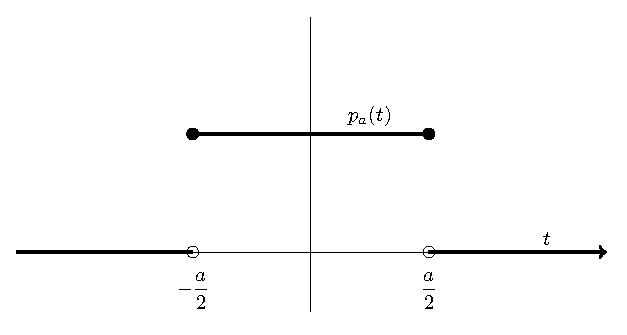
\includegraphics[scale=1]{Imagenes/funcion_paso.eps}
    \caption{Función paso rectangular.}
    \label{fig:figura_funcionpaso}
\end{figure}

Para $\omega \neq 0$ se tiene que la transformada de Fourier es:
\begin{align*}
F \big[p_{a} (\omega)\big] &= \int_{-\infty}^{\infty} p_{a}(t) \; \exp{-i \, \omega \, t} \dd{t} = \\[0.5em]
&= \scaleint{6ex}_{\bs -a/2}^{a/2} \exp(-i \, \omega \ t) \dd{t} = \left[ \dfrac{- \exp(- i \, \omega \, t)}{i \, \omega} \right] \eval_{-a/2}^{a/2} \\[0.5em]
&= \dfrac{\exp(i \, a \, \omega/2) - \exp(-i \, a \, \omega/2)}{i \, \omega} = \dfrac{2 \, \sin (a \, \omega/2)}{\omega}
\end{align*}

mientras que para $\omega = 0$, se tiene:
\begin{align*}
F \big[p_{a}(0)\big] = \int_{-\infty}^{\infty} p_{a}(t) \dd{t} = \int_{-a/2}^{a/2} \dd{t} = a
\end{align*}

Es bien sabido que el límite:
\begin{align*}
\lim_{x \to 0} \dfrac{\sin x}{x} = 1
\end{align*}

entonces obtenemos:
\begin{align*}
\lim_{\omega \to 0}  (g \, p_{a}) \, (\omega) = \lim_{\omega \to 0} \dfrac{2 \, \sin (a \, \omega /2)}{\omega} = a
\end{align*}

A pesar de que $p_{a}(t)$ en sí, no es continua, vemos que:
\begin{align}
F \big[p_{a}(\omega)\big] = \dfrac{2 \sin (a \, \omega/2)}{\omega}
\label{eq:ecuacion_06_11_Beerends}
\end{align}

es continua en $\mathbb{R}$.
\begin{figure}[H]
    \centering
    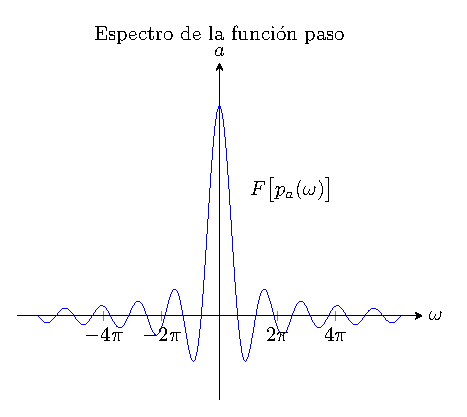
\includegraphics[scale=1]{Imagenes/T_Funcionpaso.eps}
    \caption{Transformada de Fourier de la función paso rectangular.}
    \label{fig:figura_Tfuncionpaso}
\end{figure}
% \textbf{Problema a cuenta: } Calcula la transformada de Fourier de un pulso triangular, como se muestra en la siguiente figura:
% \begin{figure}[H]
%     \centering
%     \includestandalone{Figuras/Tarea-01-Pulso_Triangular}
% \end{figure}
% \begin{align*}
% f(x) = \begin{cases}
% h(1 - a \, \abs{x}) & \abs{x} < \dfrac{1}{a} \\
% 0 & \abs{x} > \dfrac{1}{a}
% \end{cases}
% \end{align*}

\subsection*{Ejemplo. La ecuación de onda.}

Aprovecharemos la ventaja de la transformada de Fourier de la deriva para manejar ecuaciones diferenciales parciales. Consideremos una cuerda infinita que vibra, la amplitud $y$ de las vibraciones es pequeña, y satisface la ecuación de onda:
\begin{equation}
\pdv[2]{y}{x} = \dfrac{1}{v^{2}} \, \pdv[2]{y}{t}
\label{eq:ecuacion_15_42}
\end{equation}

con la condición inicial:
\begin{equation}
y(x, 0) = f(x)
\label{eq:ecuacion_15_43}
\end{equation}

donde $f$ está localizada, es decir, tiende a cero para valores grandes de $x$.
\par
Aplicar la transformada de Fourier en $x$, significa multiplicar por $\exp(i \, \omega \, x)$ y luego integrar sobre $x$, así que:
\begin{align}
\scaleint{6ex}_{\bs -\infty}^{\infty} \pdv[2]{y(x, t)}{x} \; \exp(i \, \omega \, x) \dd{x} = \dfrac{1}{v^{2}} \, \scaleint{6ex}_{\bs -\infty}^{\infty} \pdv[2]{y (x, t)}{t} \; \exp(i \, \omega \, x) \dd{x}
\label{eq:ecuacion_15_44}
\end{align}

o que es lo mismo:
\begin{equation}
(-i \, \alpha)^{2} \; Y(\alpha, t) = \dfrac{1}{v^{2}} \; \pdv[2]{Y(\alpha, t)}{t}
\label{eq:ecuacion_15_45}
\end{equation}

donde se ha utilizado:
\begin{equation}
Y(\alpha, t) = \dfrac{1}{\sqrt{2 \pi}} \scaleint{6ex}_{\bs -\infty}^{\infty} y(x, t) \; e^{i \alpha x} \, \dd x
\label{eq:ecuacion_15_46}
\end{equation}

Nótese que parte del integrando se anula: la onda aún no se ha desplazado a $\pm \infty$ porque se está propagando hacia adelante en el tiempo, y no hay una fuente en el infinito porque $f(\pm \infty) = 0$.
\par
Dado que no se tienen derivadas con respecto a $\alpha$, la ec. (\ref{eq:ecuacion_15_45}) es un EDO, de hecho la \emph{ecuación del oscilador armónico}. La transformación de una EDP a una EDO es un logro significativo. Resolvemos la ec. (\ref{eq:ecuacion_15_45}) sujeta a las condiciones iniciales. En $t=0$, aplicando las ecuaciones (\ref{eq:ecuacion_15_43}) y (\ref{eq:ecuacion_15_46}), se simplifica a:
\begin{align}
Y(\alpha, 0) = \dfrac{1}{\sqrt{2 \pi}} \int_{-\infty}^{\infty} f(x) \; e^{i \alpha x} \, \dd x =  F(\alpha)
\label{eq:ecuacion_15_47}
\end{align}
La solución general de la ec. (\ref{eq:ecuacion_15_45}) es de una forma exponencial:
\begin{align}
Y(\alpha, t) = F(\alpha) \; \exp(\pm  i \, v \, \alpha \, t)
\label{eq:ecuacion_15_48}
\end{align}
Usando la fórmula de inversión, se tiene:
\begin{align}
y(x,t) = \dfrac{1}{\sqrt{2 \, \pi}} \int_{-\infty}^{\infty} Y(\alpha, t) \; \exp(-i \, \alpha \, x) \dd{\alpha}
\label{eq:ecuacion_15_49}
\end{align}
y, por la ecuación (\ref{eq:ecuacion_15_48}):
\begin{align}
y(x, t) = \dfrac{1}{\sqrt{2 \, \pi}} \int_{-\infty}^{\infty} F(\alpha) \; \exp(- i \, \alpha (x \mp v \, t)) \dd{\alpha}
\label{eq:ecuacion_15_50}
\end{align}
Ya que $f(x)$ es la transforma inversa de Fourier de $F(\alpha)$
\begin{align}
y(x, t) = f (x \pm v \, t)
\label{eq:ecuacion_15_51}
\end{align}
que corresponde a ondas que avanzan en las direcciones $+x$ y $-x$ respectivamente.

\subsection*{Ejemplo. Ecuación de calor.}

Para nuevamente ejemplificar la transformación de una EDP a una EDO, usemos la transformada de Fourier a la EDP de flujo de calor:
\begin{align*}
\pdv{\psi}{t} = a^{2} \; \pdv[2]{\psi}{x}
\end{align*}

donde la solución $\psi(x,t)$ es la temperatura en el espacio como función del tiempo. Tomando la transformada de Fourier en ambos lados de la ecuación, nótese que $\omega$ es la variable conjugada compleja para $x$ ya que $t$ es el tiempo en la EDP de flujo de calor, donde:
\begin{align*}
\Psi(\omega, t) = \dfrac{1}{\sqrt{2 \, \pi}} \int_{-\infty}^{\infty} \psi(x, t) \; \exp(i \, \omega \, x) \dd{x}
\end{align*}

Esto nos lleva a una EDO para la transformada de Fourier $\Psi$ de $\psi$ en la variable temporal $t$:
\begin{align*}
\pdv{\Psi(\omega, t)}{t} = -a^{2} \, \omega^{2} \, \Psi(\omega, t)
\end{align*}

Al integrar, obtenemos:
\begin{align*}
\ln \Psi = -a^{2} \, \omega^{2} \, t + \ln C \hspace{1.5cm} \text{ o } \hspace{1.5cm} \Psi = C \; \exp(-a^{2} \, \omega^{2} \, t)
\end{align*}

donde la constante de integración $C$ dependerá de $\omega$ y en general queda determinada por las condiciones iniciales. De hecho $C = \Psi(\omega, 0)$ es la distribución espacial inicial de $\Psi$, que está dada por la transformación (en $x$) de la distribución inicial de $\psi$, llamada $\psi(x,0)$.
\par
Dejando la solución en la transformada inversa de Fourier, se obtiene
\begin{align*}
\psi(x, t) = \dfrac{1}{\sqrt{2 \pi}} \int_{-\infty}^{\infty} C(\omega) \; \exp(-i \, \omega \, x) \; \exp(-a^{2} \, \omega^{2} \, t) \, \dd{\omega}
\end{align*}

Por razones de simplicidad, tomamos $C$ independiente de $\omega$ (suponiendo una distribución inicial de temperatura como una función delta), al integrar completando el cuadrado en $\omega$ y realizando los cambios de variable ($a^{2} \to a^{2} \, t$, $\omega \to x$, $t \to -\omega$. Nos encontramos con una solución particular de la EDP de flujo de calor
\begin{align*}
\psi(x,t) = \dfrac{C}{a \sqrt{2 t}} \; \exp \left( - \dfrac{x^{2}}{4 \, a^{2} \, t} \right)
\end{align*}

\end{document}